\documentclass[11pt,letterpaper]{article}
\textwidth 6.5in
\textheight 9.in
\oddsidemargin 0in
\headheight 0in
\usepackage{graphicx}
\usepackage{fancybox}
\usepackage[utf8]{inputenc}
\usepackage{epsfig,graphicx}
\usepackage{multicol,pst-plot}
\usepackage{pstricks}
\usepackage{amsmath}
\usepackage{amsfonts}
\usepackage{amssymb}
\usepackage{eucal}
\usepackage[left=2cm,right=2cm,top=2cm,bottom=2cm]{geometry}
\usepackage{enumitem}
\usepackage{setspace}
\pagestyle{empty}
\DeclareMathOperator{\tr}{Tr}
\newcommand*{\op}[1]{\check{\mathbf#1}}
\newcommand{\bra}[1]{\langle#1 |}
\newcommand{\ket}[1]{| #1 \rangle}
\newcommand{\braket}[2]{\langle#1 | #2 \rangle}
\newcommand{\mean}[1]{\langle#1 \rangle}
\newcommand{\opvec}[1]{\check{\vec#1}}
% \renewcommand{\sp}[1]{$${\begin{split} #1 \end{split}}$$}
\renewcommand{\theenumi}{\Alph{enumi}}
\renewcommand{\baselinestretch}{1}

\numberwithin{equation}{section}

\usepackage{lipsum}

\usepackage{listings}
\usepackage{color}

\definecolor{codegreen}{rgb}{0,0.6,0}
\definecolor{codegray}{rgb}{0.5,0.5,0.5}
\definecolor{codepurple}{rgb}{0.58,0,0.82}
\definecolor{backcolour}{rgb}{0.95,0.95,0.92}

\lstdefinestyle{mystyle}{
	backgroundcolor=\color{backcolour},   
	commentstyle=\color{codegreen},
	keywordstyle=\color{magenta},
	numberstyle=\tiny\color{codegray},
	stringstyle=\color{codepurple},
	basicstyle=\footnotesize,
	breakatwhitespace=false,         
	breaklines=true,                 
	captionpos=b,                    
	keepspaces=true,                 
	numbers=left,                    
	numbersep=5pt,                   
	showspaces=false,                
	showstringspaces=false,
	showtabs=false,                  
	tabsize=2
}

\lstset{style=mystyle}

\begin{document}
\pagestyle{plain}

\begin{flushleft}
Student Name: LIANG, Yuchen\\
Student ID: 20582717\\
Email: yuchen.liang@connect.ust.hk
\end{flushleft}

\begin{flushright}\vspace{-19mm}
COMP5212: Machine Learning \\
Fall 2022 \\
Due Wednesday Nov. 9, 11:59 PM
\end{flushright}
 
\begin{center}\vspace{0.2cm}
\textbf{\LARGE Programming Homework 2}\\
Homework Report
\end{center}

\rule{\linewidth}{0.5mm}
%%%%%%%%%%%%%%%%%%%%%%%%%%%%%%%%%%%%%%%%%%%%%%%%%%%%%%%%%%%%%%%%%%%%%%%%

% \bigskip
% \bigskip

%%%%%%%%%%%%%%%%%%%%
%%%%%%%%%%%%%%%%%%%%
\section{Convolutional neural network (MLP) Implementation}
\subsection{Model Description}
The model is a 7 layers fully-connected neural networks with ReLU activation function.
\subsection{Implementation Details}
The model details are shown below:
\begin{lstlisting}
    Batch size = 64
    Number of epochs = 20
    self.model = nn.Sequential(
            nn.Flatten(),
            nn.Linear(3072, 1024),  nn.ReLU(),
            nn.Linear(1024, 512),   nn.ReLU(),
            nn.Linear(512, 256),    nn.ReLU(),
            nn.Linear(256, 128),    nn.ReLU(),
            nn.Linear(128, 64),     nn.ReLU(),
            nn.Linear(64, 32),      nn.ReLU(),
            nn.Linear(32, 10),      nn.ReLU(),
    )
\end{lstlisting}

\subsection{Training Results}
\begin{lstlisting}
    Total accuracy:               53%
    |   plane   class accuracy:   65.8%
    |   car     class accuracy:   68.8%
    |   bird    class accuracy:   31.2%
    |   cat     class accuracy:   33.3%
    |   deer    class accuracy:   32.8%
    |   dog     class accuracy:   40.5%
    |   frog    class accuracy:   58.6%
    |   horse   class accuracy:   72.7%
    |   ship    class accuracy:   62.8%
    |   truck   class accuracy:   69.1%
\end{lstlisting}


\newpage

%%%%%%%%%%%%%%%%%%%%
%%%%%%%%%%%%%%%%%%%%
\section{Multilayer perceptron (CNN) Implementation}
\subsection{Model Description}
The model is a 7 layers convolutional neural networks, 4 convolutional layers and 3 fully-
connected layers, with ReLu activation function.
\subsection{Implementation Details}
The model details are shown below:
\begin{lstlisting}
    Batch size = 64
    Number of epochs = 20
    self.model = nn.Sequential(
            nn.Conv2d(3,64,3, stride=1, padding=1),     nn.ReLU(),
            nn.Conv2d(64,128,3, stride=2, padding=1),   nn.ReLU(),
            nn.Conv2d(128,256,3, stride=2, padding=1),  nn.ReLU(),
            nn.Conv2d(256,256,3, stride=2, padding=1),  nn.ReLU(),
            nn.Flatten(),
            nn.Linear(4096, 1024),      nn.ReLU(),
            nn.Linear(1024, 1024),      nn.ReLU(),
            nn.Linear(1024, 10),
        )
\end{lstlisting}

\subsection{Training Results}
\begin{lstlisting}
    Total accuracy:               82%
    |   plane   class accuracy:   91.1%
    |   car     class accuracy:   91.4%
    |   bird    class accuracy:   72.0%
    |   cat     class accuracy:   58.1%
    |   deer    class accuracy:   81.7%
    |   dog     class accuracy:   77.8%
    |   frog    class accuracy:   86.7%
    |   horse   class accuracy:   87.5%
    |   ship    class accuracy:   89.1%
    |   truck   class accuracy:   87.7%
\end{lstlisting}


\newpage

%%%%%%%%%%%%%%%%%%%%
%%%%%%%%%%%%%%%%%%%%
\section{Discussion}
\subsection{Compare of MLP and CNN}
The comparison of the average training loss of using MLP and CNN is shown in Figure \ref{fig:loss}.
\begin{figure}[htbp]
    \centering
    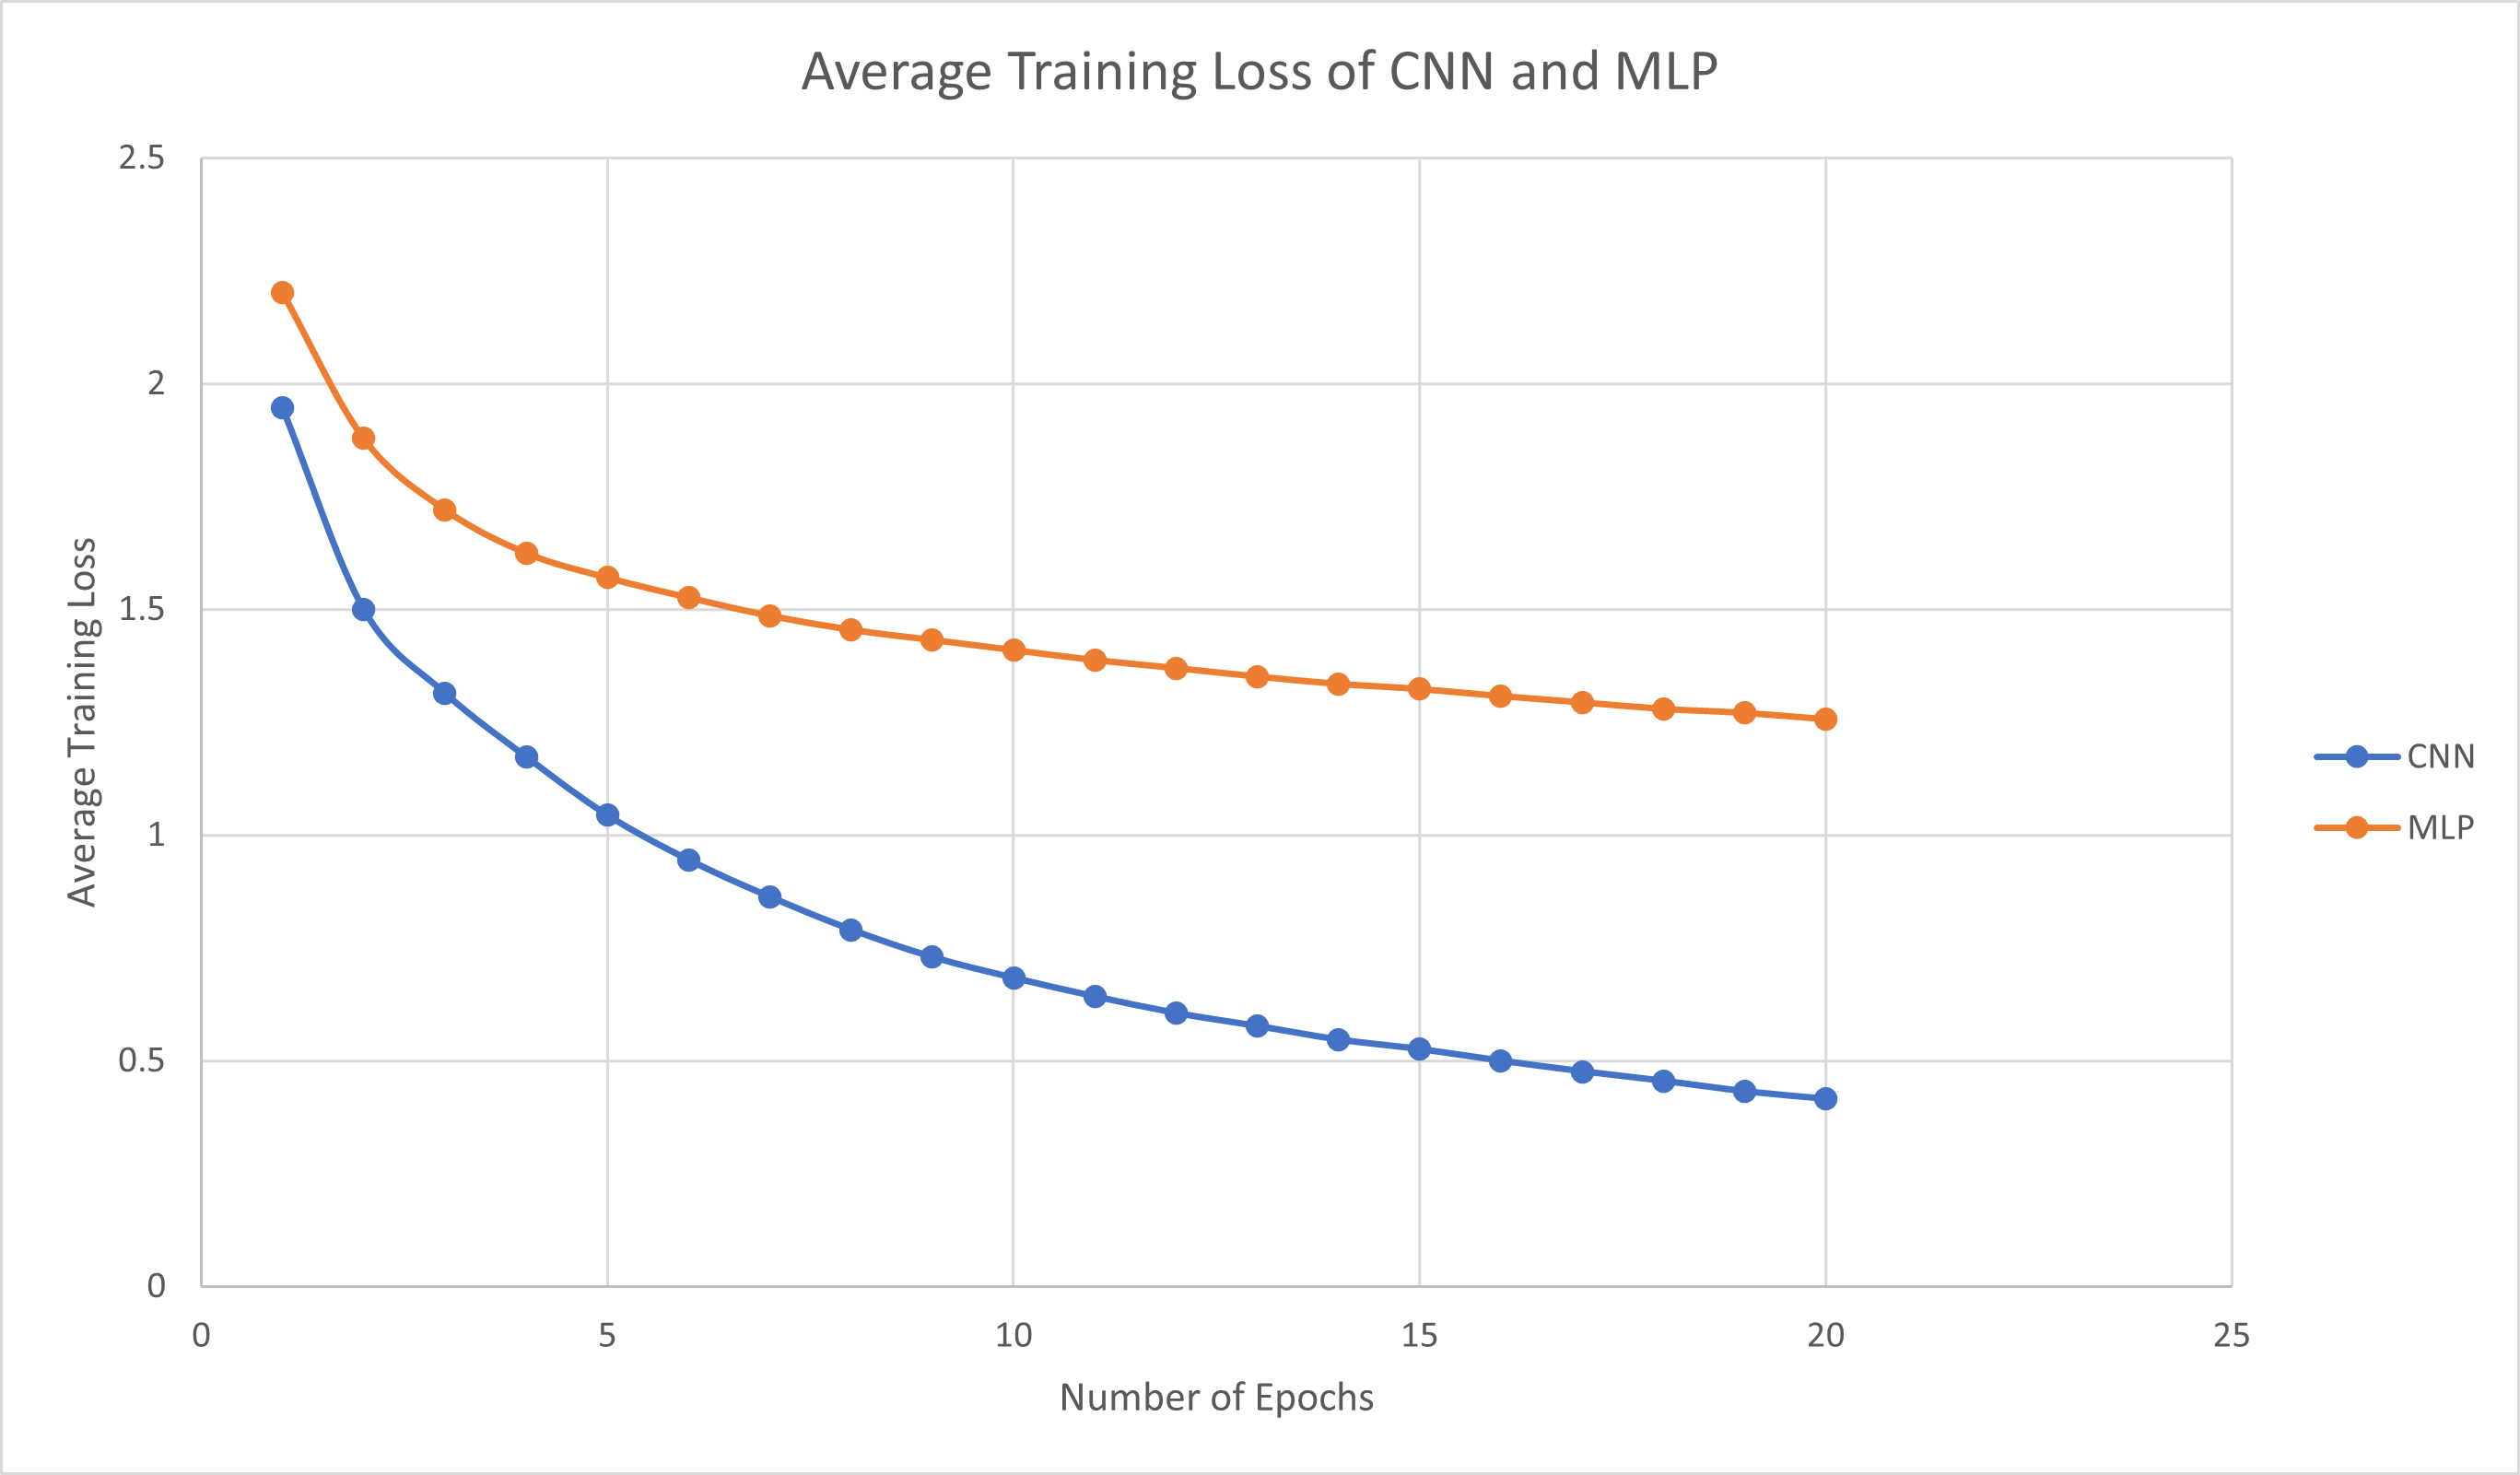
\includegraphics[width=0.6\linewidth]{./assets/AVGLOSS.png}
    \caption{Loss Comparison}
    \label{fig:loss}
\end{figure}
From the figure, it is shown that the loss of CNN is smaller than MLP, therefore we can infer that the CNN is more efficient than MLP.


\subsection{Neural network with and without non-linear activation function}
This report implement model without non-linear activation function on MLP and compare. The result is shown in Figure \ref{fig:relu}.
\begin{figure}[htbp]
    \centering
    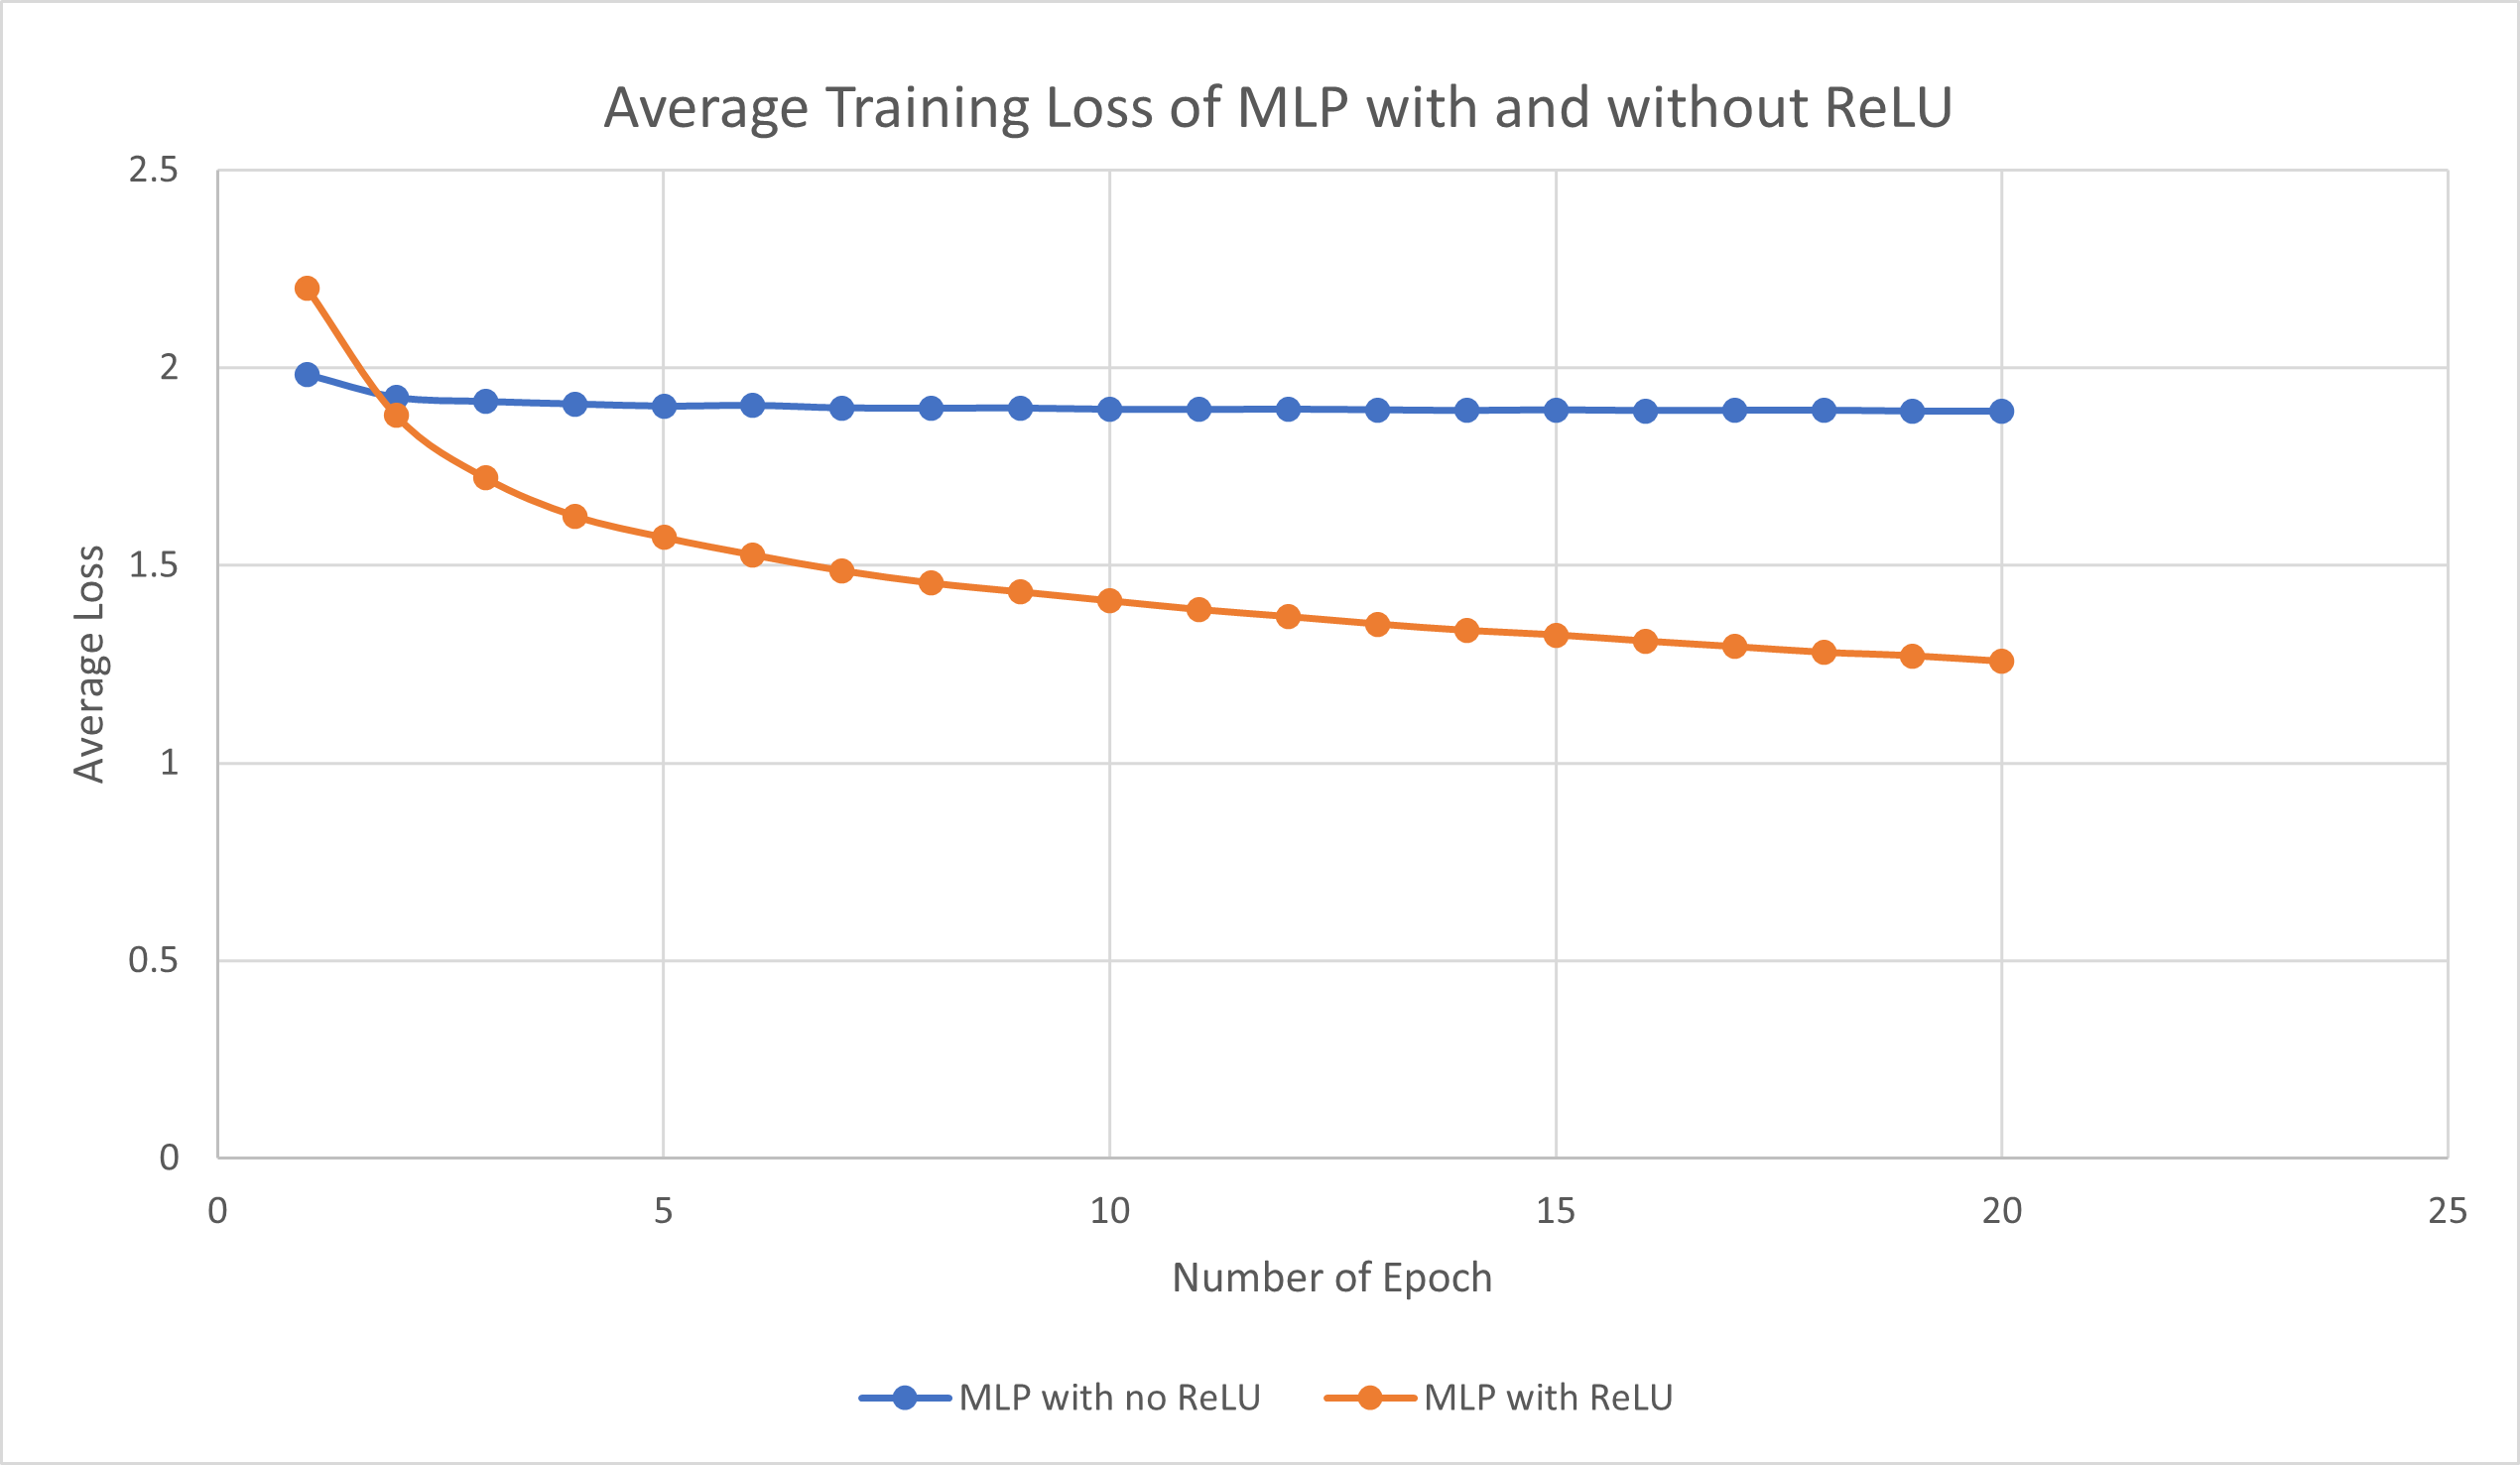
\includegraphics[width=0.6\linewidth]{./assets/AVGLOSSRELU.png}
    \caption{with and without non-linear activation function}
    \label{fig:relu}
\end{figure}
The model without non-linear activation function is not able to converge. The model with non-linear activation function is able to converge and get better result.

\end{document}
